\documentclass{beamer}
\usepackage[utf8]{inputenc}

\usetheme{Madrid}
\usecolortheme{default}
\usepackage{amsmath,amssymb,amsfonts,amsthm}
\usepackage{tkz-euclide}
\usepackage{listings}
\usepackage{adjustbox}
\usepackage{array}
\usepackage{tabularx}
\usepackage{gvv}
\usepackage{lmodern}
\usepackage{circuitikz}
\usepackage{tikz}
\usepackage{graphicx}

\setbeamertemplate{page number in head/foot}[totalframenumber]

\usepackage{tcolorbox}
\tcbuselibrary{minted,breakable,xparse,skins}



\definecolor{bg}{gray}{0.95}
\DeclareTCBListing{mintedbox}{O{}m!O{}}{%
  breakable=true,
  listing engine=minted,
  listing only,
  minted language=#2,
  minted style=default,
  minted options={%
    linenos,
    gobble=0,
    breaklines=true,
    breakafter=,,
    fontsize=\small,
    numbersep=8pt,
    #1},
  boxsep=0pt,
  left skip=0pt,
  right skip=0pt,
  left=25pt,
  right=0pt,
  top=3pt,
  bottom=3pt,
  arc=5pt,
  leftrule=0pt,
  rightrule=0pt,
  bottomrule=2pt,
  toprule=2pt,
  colback=bg,
  colframe=orange!70,
  enhanced,
  overlay={%
    \begin{tcbclipinterior}
    \fill[orange!20!white] (frame.south west) rectangle ([xshift=20pt]frame.north west);
    \end{tcbclipinterior}},
  #3,
}
\lstset{
    language=C,
    basicstyle=\ttfamily\small,
    keywordstyle=\color{blue},
    stringstyle=\color{orange},
    commentstyle=\color{green!60!black},
    numbers=left,
    numberstyle=\tiny\color{gray},
    breaklines=true,
    showstringspaces=false,
}
\usepackage[utf8]{inputenc}
\usepackage[T1]{fontenc}



%------------------------------------------------------------
%This block of code defines the information to appear in the
%Title page
\title %optional
{1.2.11}
\date{August 21,2025}
%\subtitle{A short story}

\author % (optional)
{Megha Shyam-AI25BTECH11005}




\begin{document}


\frame{\titlepage}
\begin{frame}{Question}
 Find the slope of lines
\begin{enumerate}
    \item Passing through the points $(3, -2)$ and $(-1, 4)$
    \item Passing through the points $(3, -2)$ and $(7, -2)$
    \item Passing through the points $(3, -2)$ and $(3, 4)$
    \item Making inclination of $60^\circ$ with the positive direction of $x$-axis
\end{enumerate}
\end{frame}



\begin{frame}{Theoretical Solution}
\textbf{Finding slopes using the direction vector formula}

The direction vector of \(AB\) is defined as  
\[
\mathbf{m} = \mathbf{B} - \mathbf{A} = \kappa \begin{pmatrix}1 \\ m \end{pmatrix},
\]  
where \(m\) is the slope of \(AB\).  
We also write  
\[
\mathbf{m} \equiv \begin{pmatrix}1 \\ m \end{pmatrix}.
\]  
Hence, the slope \(m\) can be obtained directly from the direction vector components:
\[
m = \frac{\text{vertical component of }(\mathbf{B}-\mathbf{A})}
         {\text{horizontal component of }(\mathbf{B}-\mathbf{A})}.
\]

---
\end{frame}
\begin{frame}{Theoritical Solution}
    



   \textbf{Through points \((3,-2)\) and \((-1,4)\):}  

  Let  
  \[
  \mathbf{A}=\begin{pmatrix}3\\-2\end{pmatrix},\quad
  \mathbf{B}=\begin{pmatrix}-1\\4\end{pmatrix}.
  \]  
  The direction vector is  
  \[
  \mathbf{B}-\mathbf{A}
    =\begin{pmatrix}-1-3\\4-(-2)\end{pmatrix}
    =\begin{pmatrix}-4\\6\end{pmatrix}.
  \]  
  Comparing with \(\kappa\begin{pmatrix}1\\m\end{pmatrix}\),  
  \[
  m = \frac{6}{-4} = -\frac{3}{2}.
  \]
  
\end{frame}
\begin{frame}{Theoritical Solution}
  \textbf{Through points \((3,-2)\) and \((7,-2)\):}  

  \[
  \mathbf{A}=\begin{pmatrix}3\\-2\end{pmatrix},\quad
  \mathbf{B}=\begin{pmatrix}7\\-2\end{pmatrix},
  \]  
  \[
  \mathbf{B}-\mathbf{A}
    =\begin{pmatrix}7-3\\-2-(-2)\end{pmatrix}
    =\begin{pmatrix}4\\0\end{pmatrix},
  \]  
  so  
  \[
  m = \frac{0}{4}=0.
  \]
  \end{frame}
  \begin{frame}{Theoritical Solution}
      
 
   \textbf{Through points \((3,-2)\) and \((3,4)\):}  

  \[
  \mathbf{A}=\begin{pmatrix}3\\-2\end{pmatrix},\quad
  \mathbf{B}=\begin{pmatrix}3\\4\end{pmatrix},
  \]  
  \[
  \mathbf{B}-\mathbf{A}
    =\begin{pmatrix}3-3\\4-(-2)\end{pmatrix}
    =\begin{pmatrix}0\\6\end{pmatrix},
  \]  
  here the horizontal component is zero, so  
  \[
  m = \frac{6}{0},
  \]  
  which is undefined (vertical line).
  \end{frame}
  \begin{frame}{Theoritical Solutions}
      
  

  \textbf{Inclination of \(60^\circ\) with the positive \(x\)-axis:}  

  A direction vector making an angle \(\theta\) with the \(x\)-axis is  
  \[
  \mathbf{m}=\begin{pmatrix}\cos\theta \\ \sin\theta\end{pmatrix}
    =\kappa\begin{pmatrix}1\\\tan\theta\end{pmatrix},
  \]  
  so  
  \[
  m=\tan60^\circ=\sqrt{3}.
  \]






\end{frame}
\begin{frame}[fragile]{C code}
\begin{lstlisting}[language=C]
#include <stdio.h>
int main() {
    double Ax, Ay, Bx, By, dx, dy, slope;
    printf("Enter coordinates of point A (x y): ");
    scanf("%lf %lf", &Ax, &Ay);
      printf("Enter coordinates of point B (x y): ");
     scanf("%lf %lf", &Bx, &By); 
     dx = Bx - Ax; // horizontal component
    dy = By - Ay; // vertical component
    if (dx == 0) {
        printf("The line AB is vertical. The slope is undefined (infinite).\n");
    } else {
        slope = dy / dx;
        printf("Direction vector of AB: (%.2f, %.2f)\n", dx, dy);
        printf("Slope of AB: %.2f\n", slope);
    }
 return 0;
}
\end{lstlisting}
\end{frame}
\begin{frame}[fragile]
\frametitle{\textbf{Python Plotting Code - Part 1}}
\begin{lstlisting}[language=Python]
import matplotlib.pyplot as plt
import numpy as np

# Points
A = (3, -2)
B1 = (-1, 4)
B2 = (7, -2)
B3 = (3, 4)

# 1) Line through (3,-2) & (-1,4)
x1 = np.linspace(-2, 5, 100)
m1 = (4 - (-2)) / (-1 - 3)  # slope = -1.5
y1 = m1 * (x1 - 3) + (-2)

# 2) Horizontal line through (3,-2) & (7,-2)
x2 = np.linspace(-2, 8, 100)
y2 = np.full_like(x2, -2)
\end{lstlisting}
\end{frame}
\begin{frame}[fragile]
\frametitle{\textbf{Python Plotting Code - Part 2}}
\begin{lstlisting}[language=Python]
# 3) Vertical line through (3,-2) & (3,4)
x3 = np.full(100, 3)
y3 = np.linspace(-3, 5, 100)

# 4) Line with inclination 60' (slope = tan(60') 1.732) through origin
x4 = np.linspace(-2, 4, 100)
m4 = np.tan(np.radians(60))
y4 = m4 * x4

# Plot all lines
plt.plot(x1, y1, 'orange', label="Through (3,-2) & (-1,4); slope = -1.50")
plt.plot(x2, y2, 'blue', label="Through (3,-2) & (7,-2); slope = 0")
plt.plot(x3, y3, 'green', label="Through (3,-2) & (3,4); vertical (undefined slope)")
plt.plot(x4, y4, 'gold', label="Inclination 60'; slope = 1.732")
\end{lstlisting}
\end{frame}
\begin{frame}[fragile]
\frametitle{\textbf{Python Plotting Code - Part 3}}
\begin{lstlisting}[language=Python]
# Points
plt.scatter([3, -1, 7, 3, 0], [-2, 4, -2, 4, 0], color='black', zorder=5)
plt.text(3, -2.4, "(3,-2)")
plt.text(-1.5, 4, "(-1,4)")
plt.text(7, -2.4, "(7,-2)")
plt.text(3.1, 4, "(3,4)")
plt.text(0.1, 0.2, "(0,0)")

# Labels and grid
plt.title("Lines and Slopes from the Problem")
plt.xlabel("x")
plt.ylabel("y")
plt.axhline(0, color='black', linewidth=0.8)
plt.axvline(0, color='black', linewidth=0.8)
plt.grid(True)
plt.legend()
plt.show()
\end{lstlisting}
\end{frame}
\begin{frame}{Plot}
 \begin{figure}[H]
     \centering
     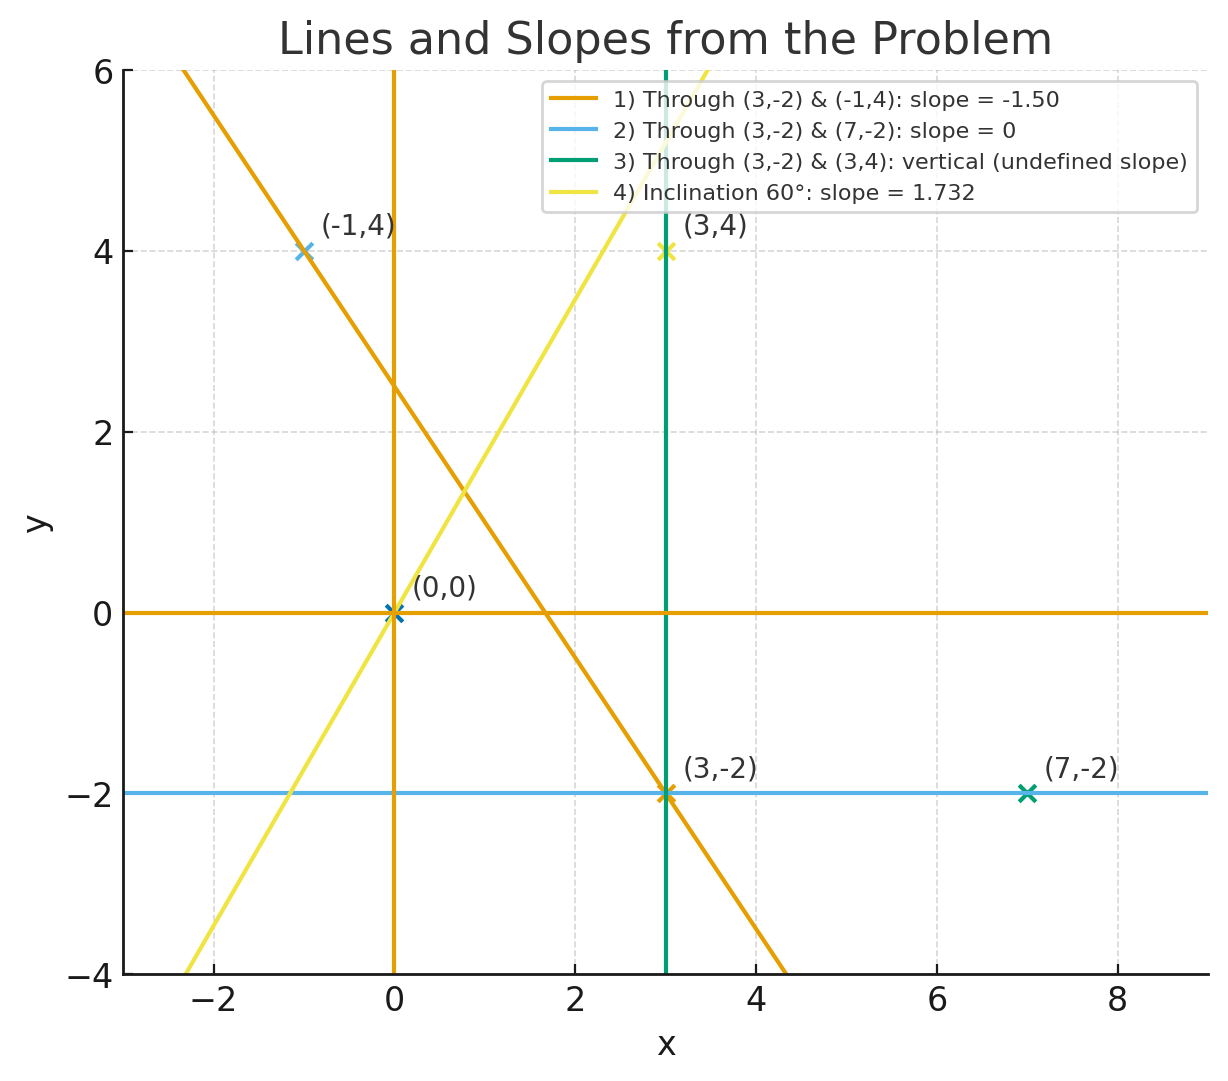
\includegraphics[width=0.5\linewidth]{figs/fig1.png}
     \caption{fig1}
     \label{fig:placeholder}
 \end{figure}
     
    
\end{frame}


\end{document}